%%% template.tex
%%%
%%% This LaTeX source document can be used as the basis for your technical
%%% paper or abstract. Regardless of the length of your document, the commands
%%% are all the same.
%%% 
%%% The "\documentclass" command is the first command in your file. If you want to 
%%% prepare a version of your article with line numbers - a "review" version - 
%%% include the "review" parameter:
%\usepackage{mathrsfs}

\documentclass[review]{acmsiggraph}
%%%
\usepackage{amssymb}

\usepackage{graphicx}
\usepackage{subfigure}

%%%\documentclass{acmsiggraph}

%%% Title of your article or abstract.

\title{FoldingBox: From 2D Layout to 3D Model???}

\author{XX\thanks{e-mail:XX}\\Chair, ACM SIGGRAPH Publications Committee}
\pdfauthor{XX}

%%% Used by the ``review'' variation; the online ID will be printed on 
%%% every page of the content.

\TOGonlineid{XX}

% User-generated keywords.

\keywords{3D Model?, XX}

% With the "\setcopyright" command the appropriate rights management text will be added
% to your document.

%\setcopyright{none}
%\setcopyright{acmcopyright}
%\setcopyright{acmlicensed}
\setcopyright{rightsretained}
%\setcopyright{usgov}
%\setcopyright{usgovmixed}
%\setcopyright{cagov}
%\setcopyright{cagovmixed}
%\setcopyright{rightsretained}

% The year of publication in the "\copyrightyear" command.

\copyrightyear{2017}

%%% Conference information, from the completed rights management form.
%%% The "\conferenceinfo" command has two parameters: 
%%%    - conference name
%%%    - conference date and location
%%% The "\isbn" field includes the year and month after the article ISBN.

\conferenceinfo{SIGGRAPH 2017 Posters}{XX, 2017, XX, XX} 
\isbn{XX} 
\doi{XX}

\begin{document}

%%% This is the ``teaser'' command, which puts an figure, centered, below 
%%% the title and author information, and above the body of the content.

 \teaser{
   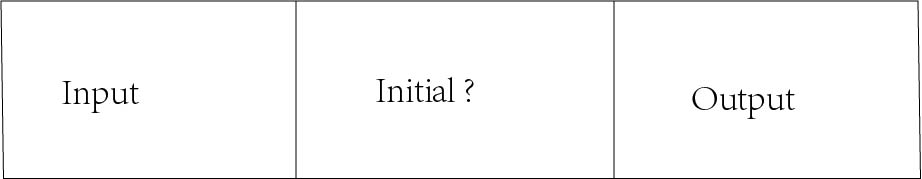
\includegraphics[height=1.4in]{images/teaser.jpg}
   \caption{\textbf{Overview.} (a) A given input layout (b) XX (c) final 3D model generated by our methods}
 }

\maketitle

\begin{abstract}

In this paper, we will propose a new method for generating 3D models given its 2D layout, whose folded angels are learnt(?) by XX optimization. 

\end{abstract}

%
% The code below should be generated by the tool at
% http://dl.acm.org/ccs.cfm
% Please copy and paste the code instead of the example below. 
%

%\begin{CCSXML}
%<ccs2012>
%<concept>
%<concept_id>10010147.10010371.10010382</concept_id>
%<concept_desc>Computing methodologies~Image manipulation</concept_desc>
%<concept_significance>500</concept_significance>
%</concept>
%<concept>
%<concept_id>10010147.10010371.10010382.10010236</concept_id>
%<concept_desc>Computing methodologies~Computational photography</concept_desc>
%<concept_significance>300</concept_significance>
%</concept>
%</ccs2012>
%\end{CCSXML}

%\ccsdesc[500]{Computing methodologies~Image manipulation}
%\ccsdesc[300]{Computing methodologies~Computational photography}

%
% End generated code
%

% The next three commands are required, and insert the user-generated keywords, 
% The CCS concepts list, and the rights management text.
% Please make sure there is a blank line between each of these three commands.

\keywordlist

\conceptlist

\printcopyright

\section{Introduction}
Cartons have been widely used in packaging industry, to deliver various commodities including food items, daily necessities and electronic components. Instead of very basic packaging shapes like cubes, there exist multiple fantastic cartons to package wedding candies or take away coffee. These various designs increase much popularity, not to mention they're environment friendly due to their recycling and degradability.

{\color{red}{Cartons are usually designed based on experience and trial-and-error?}} Depressingly,  designers cannot see directly final model of carton when they are drawing its layout. Moreover, for  non-experts, it's intractable to fold an irregular layout to final carton without instructions.

Researchers have studied paper folding problem for more than twenty years. It's been verified that  given a net, i.e., a polygon and a set of creases, and the dihedral angles at each crease, we can know whether a polyhedron can be obtained in polynomial time. However, if the dihedral angles stay unknown, this problem becomes NP-hard even we simplify the 3D mdoel to orthogonal polyhedron whose dihedral angles are multiples of $\pi/2$ \cite{Biedl:2005:NFP:1090462.1646553}.

However, the study above more focused on academic fileds, not on the applications of practical use. 

Three-dimensional reconstruction has been wildly studied from different sources, such as point clouds, single images, and line drawings. 
 
\section{Related Work}
\textbf{Reconsturction from single line drawings.} Line drawings of three-dimensional objects have long been studied, and the main problem is still in reconstruction given projection on two-dimensional planes. Some researchers treat this task as optimization problem. \cite{Marill:1991:EHI:113057.113061} proposed MSDA(Minimize the Standard Deviation of Angles) principle to emulate the interpretion of line drawings as 3D objects. This new criterion is used by many other researchers later. \cite{Leclerc1992An} combined MSDA with the deviation from planarity as objective terms. \cite{Cao:2005:ORS:1097114.1097658} added symmetry measure of the objects to get more complicated results. Some other researchers try to solve this problem from the information theoretic point of view. \cite{Marill1992Why} minimized the description length of objects based on the idea that we usually pick the simplest one from infinite possibilities when we see the line drawing. \cite{Shoji20013} implemented the principle of minimizing the entropy of angle distribution between line segments using genetic algorithm. Different from the input above, ours are expanded layout of three-dimensional objects in 2D planes, the lackness of 3D topology is main cencern in our problem.

\textbf{Folding to polyhedron.} \cite{Lubiw1996When} provided an dynamic programming algorithm based on Aleksandrov's theorem to test whether a polygon can be folded into polyhedra which takes $O(n^2)$ time and space. \cite{O'Rourke:1998:FUC:646319.686376} examined three open problems on the subject of folding and unfolding. \cite{Biedl2004When} has studied in polynomial time to solve the question of when is the graph  orthogonally convex polyhedra given a graph, edge length and facial angles, also shown that it's NP-hard to decide whether the graph is orthogonally polyhedra or not. Rather than given graph, \cite{Biedl:2005:NFP:1090462.1646553} proved that if given a net along with the dihedral angle at each crease, we can know whether a net can be folded to a polyhedron in polynomial time, but it becomes NP-hard without the angles even adding constrains on orthogonal polyhedron, which results in more difficultes on more complex input. Later, \cite{Demaine2010A} proposed a survey on the folding and unfolding in computational geometry. Compared to our desired result, polyhedron is a set of polygons without overlap, nevertheless, our 3D model contains paste faces that needs to be fixed to another panel. These works above justify our problem being harder to solve causing by even intricater inputs.

\textbf{Paper craft.} Various types of paper crafts have been studied in the field of computing and mathmatics. Origami is the Japanese traditional paper art of making different kind of objects by a single sheet of paper, and has been long studied since 1970s \cite{KANADE1980279}. Lately, there have been newly researched automaticly generating a type of paper architecture named pop-ups. \cite{Li:2010:PAP:1833349.1778848} presented formulation of layouts, sufficient conditions to generate foldable and stable paper architectures, and proposed an automatic algorithm given any 3D models. Plenty papers studied this subject following the idea of Li's and make new improvements\cite{Li:2011:GSV:1964921.1964993} \cite{Ruiz:2013:GMP:2542355.2542360} \cite{Le:2014:SCO:2574223.2574468}.

\textbf{Motion planning of paper folding.}

%\begin{figure*}[ht]
%	\centering
%	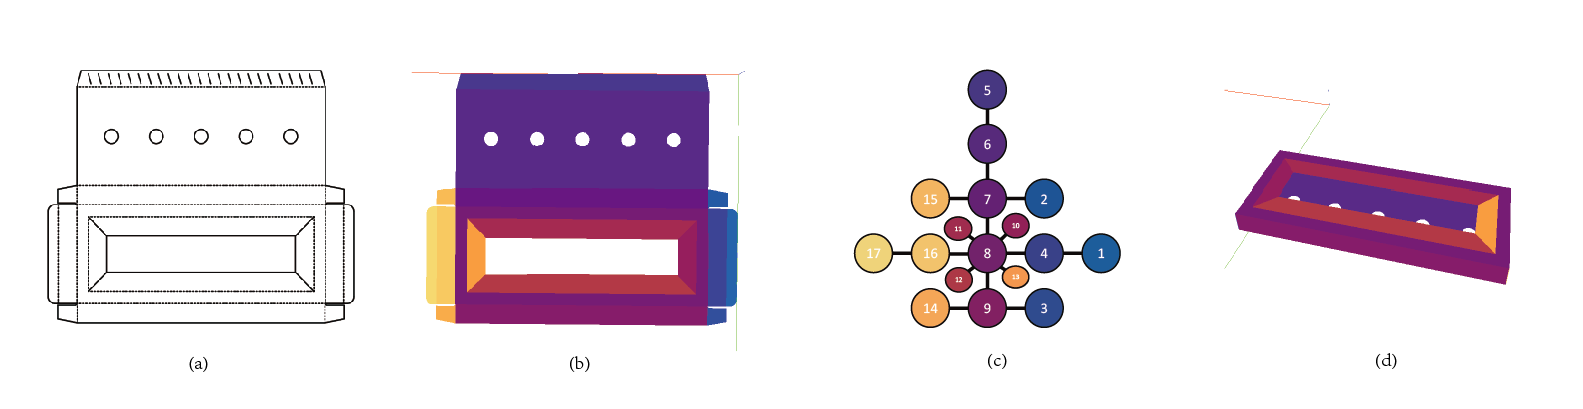
\includegraphics[width=7.0in]{images/overview.png}
%	\caption{Given input planar layout (a), we first find all its rigid plane by floodfill algorithm (b), then construct a connected graph $G$ (c), finally we have a 3D model of carton (d).}
%	\label{fig:overview}
%\end{figure*}

%\section{Formulation}
%In our paper, we take a planar layout $\mathcal{L} = \{l_1, l_2, \dots, l_N\}$ as input, where $l_i$ is the $i$th line segment, which consists of two points $P_1, P_2$ and one label, and N denotes the number of line segments. The label shows the line segment is solid or dashed which is used to cut or fold. When involving bezier curves, we sample them to short lines with a pre-defined sampling interval.
%
%To formulate our problem, we assume that every plane is rigid which means the interior angle in each plane stays the same, but planes can be bent during folding. Furthermore, planes are connected by hinges at the boundry of the patches, and we assume that the planar layout has its front and back.
%
%We first find rigid planes $\mathcal{P} = \{P_1, P_2, \dots, P_M\}$ using floodfill algorithm, then  computing the corresponding dihedral angle $\alpha_i$ between the back face of two neighbouring planes of each dashed line $l_i$ which forms the set $\mathcal{A} = \{\alpha_1, \alpha_2, \dots, \alpha_N\}$, we can reconstructe each line's three-dimensional coordinate and finally have a stable 3D model $\mathcal{M}$ of carton, where the definition of stablility is described in detail in section 3.1.
%
%\begin{figure}[ht]
%	\centering
%	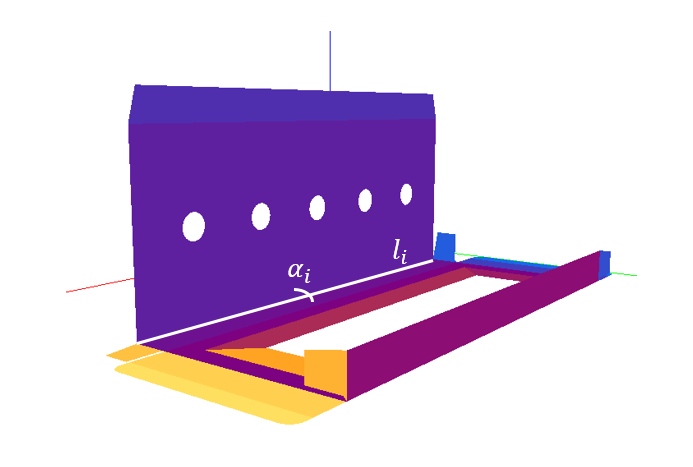
\includegraphics[width=3.0in]{images/angle.png}
%	\caption{Each fold line $l_i$ is corresponding to a folding angle $\alpha_i$ }
%	\label{fig:fold}
%\end{figure}
%
%%\subsection{Mobility in Metamorphic Mechanisms}
%%\cite{Dai1999Mobility} said in their earlier report that the carton can be represented as a mechanism model, where paper creases act as joints and paper panels act as linkage. However, the complexity of this mechanism complicates the study of mobility, so they represent metamorphic mechanism as equivalent screw system.
%%
%%Generally, the mobility formula to compute the degree of freedom of screw systems is Chebychev–Grübler–Kutzbach criterion \cite{wiki:xxx}, which is defined as 
%%
%%\begin{equation}
%% F = b(N-1-j) + \sum_{i=1}^{j} f_i 
%%\end{equation}
%%
%%where $b$ is 6 in the general spatial case and 3 in the planar case, $N$ is the total panel number, $j$ is the number of joints with freedom $f_i$, and $F$ is the freedom of the whole system.
%%
%%When a mechanism contains multiple loop linkages, the criterion evolves to equation(2).
%%
%%\begin{equation}
%% F = F_c + F_o = b(N-1-j) + j + j_o 
%%\end{equation}
%%
%%where $F_c$ is the mobility in the close loop, and $F_c$ is the mobility in the open loop, and $j_o$ is the number of joints in the open loop.
%
%\subsection{Stability}
%%To formulate stability of generated 3D model folded by given input layout, we follow the idea of computing the mobility in metamorphic mechanisms as described in section 4.2. 
%%
%%We first construct a connected graph on the input planar layout as $G = (V, E)$, which consists of a set $V = \{ \mathit{v}_{1},\cdots, \mathit{v}_{n}\}$ of $n$ nodes and a set $E = \{ \mathit{e}_{1},\cdots, \mathit{e}_{m}\}$ of $m$ edges. Each node represents a face in the layout, and there exists an edge if two nodes are adjacent.
%
%To describe stability of generated 3D model folded by given input layout, we formulate a transformation on a planar layout similar to that in \cite{Li:2011:GSV:1964921.1964993}.
%
%\textbf{Definition 1} \textit{A} \textbf{fold transform} \textit{{$f(\mathcal{L},\mathcal{A})$} on a planar layout $\mathcal{L}$ is a continuous deformation of $\mathcal{L}$ where the deformation is identity and  is a combination of rotations on each plane of $\mathcal{L}$ and the dihedral angle of the $i$th fold line is $\alpha_i \in \mathcal{A}$}.
%
%%{\color{blue}{and merging means when two planes have the same plane equation, besides the smaller plane is in the area of bigger one, then the smaller plane can be merged to the bigger one}}.
%
%We formulate a stability condition that asks the model to be stable after implementing the fold transform on the given layout to describe a stable carton that is standable and each plane has no freedom to move even given external force.
%
%\textbf{Definition 2} \textit{A fold transform $f(\mathcal{L},\mathcal{A})$ on a planar layout $\mathcal{L}$ is said to be} \textbf{stable} \textit{if all the fold angle in $\mathcal{A}$ will stay the same even given external force.}
%
%{\color{blue}{In fact, when we give a specific angle to a fold line, it won't keep static all the time, so sometimes we need glue a plane to another as Figure \ref{fig:merge}. If  two planes have the same plane equation, besides the smaller plane is in the area of bigger one, then the smaller plane can be merged to the bigger one, as in reality, we glue one face to another.}}
%
%\begin{figure}[ht]
%	\centering
%	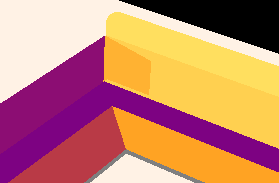
\includegraphics[width=3.0in]{images/merge.png}
%	\caption{A smaller plane merged to another to keep stability. {\color{red}{Add physical model??}}}
%	\label{fig:merge}
%\end{figure}
%
%However not every model is stable, it may has a near-stable condition that some flips can be free to rotate, the cup carrier in Figure \ref{fig:merge} is a good example. 
%
%%\textbf{Definition 3} \textit{A fold transform $f(\mathcal{L},\mathcal{A})$ on a planar layout $\mathcal{L}$ is said to be} \textbf{near-stable} \textit{if {\color{blue}{five planes of the model}}  keep stationary even given external force.}
%
%\begin{figure}[ht]
%	\centering
%	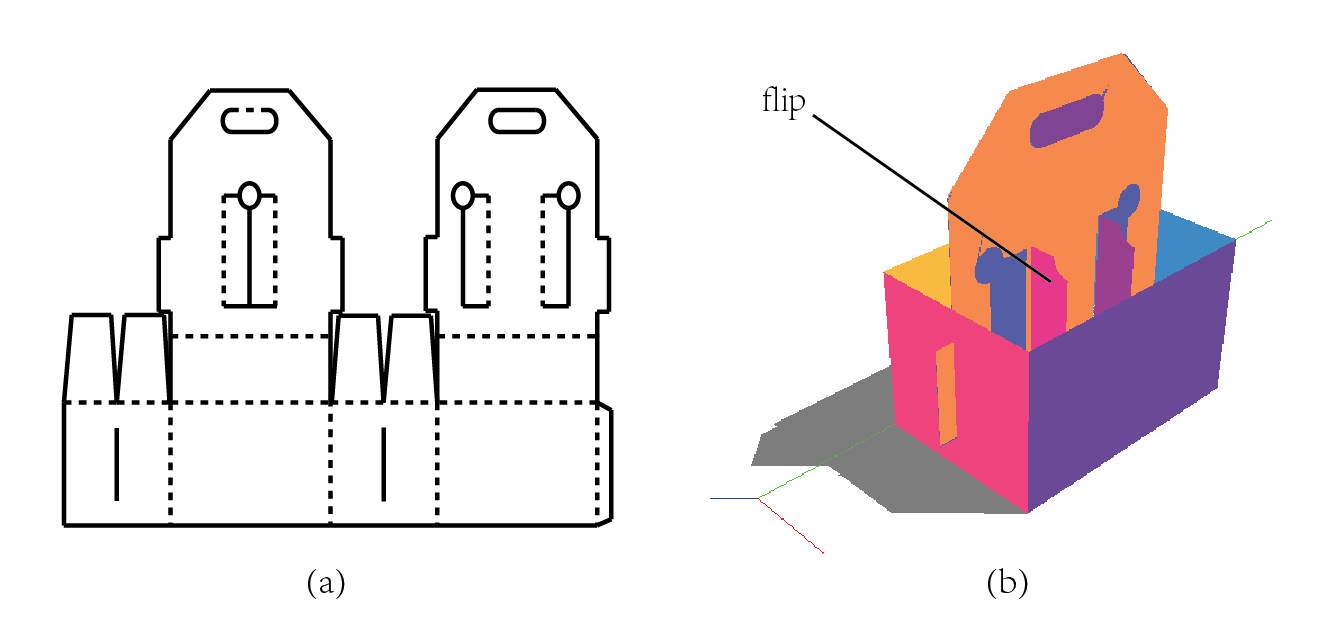
\includegraphics[width=3.0in]{images/near-stable.png}
%	\caption{Given a planar layout (a), we can generate a near-stable 3D model of cup carrier (b) whose flip between two coffee cups is free to rotate.}
%	\label{fig:near}
%\end{figure}
%
%As a consequence, we minimize the number of lines which have no given angles as our aim to construct the final 3D model as stable as possible.
%
%\begin{equation}
%f(\mathcal{A}) = n-n_{fixed}
%\end{equation}
%
%where n means the total number of fold lines, and $n_{fixed}$ denotes the number of lines that have been assigned specific angles.
%
%\subsection{Mechanism}
%Mechanism is a basic structure which is a common part of carton. Here we will introduce a few mechanisms that help us to generate 3D models of carton.
%
%\textbf{Mechanism 1} \textit{If there are three planes that form the peak of a triangular pyramid, these three planes stay stationary even given external force.}
%
%\textbf{Proof 1:} First of all, we construct three rigid planes: $P_1$, $P_2$, $P_3$, such that $P_1$ is bounded by two lines $l_1$ and $l_2$ which form an interior angle of $\theta_{12}$, $P_2$ is bounded by two lines $l_2$ and $l_3$ which form an interior angle of $\theta_{23}$, and similarly $P_3$ has two lines $l_1$ and $l_3$ which form an interior angle of $\theta_{13}$. These three planes can compose a peak of a tetrahedron with their back face inside, and intersect at point A. Furthermore, we project $l_1$ to the plane $P_2$ vertically to get line $l^{'}_1$, as we can see in Figure \ref{fig:peak}(b). We also have four unit vectors $\mathbf{l_1}$,$\mathbf{l_2}$,$\mathbf{l_3}$,$\mathbf{l_1^{'}}$ which are parallel to fold line $l_1$,$l_2$,$l_3$,$l_1^{'}$ separately.
%
%Next we need to compute the angle of $\theta_{1^{'}2}$ by construting $\overrightarrow{OC} \cdot \mathbf{l_2} = 0$ with point $C \in l_2$, and $\overrightarrow{OD} \cdot \mathbf{l_3} = 0$ with point $D \in l_3$. Now we have $\overrightarrow{BO} \perp P_2$, so that $\overrightarrow{BO} \cdot \mathbf{l_2} = 0$ and then $\mathbf{l_2} \cdot \overrightarrow{BC} = 0$, similarly, we have $\overrightarrow{BD} \cdot \mathbf{l_3} = 0$, finally we can construt simultaneous equations based on law of sines to solve the value of $\theta_{1^{'}2}$ as follows:
%
%\begin{equation}
%\left\{
%\begin{aligned}
% l_1^{'} \cos \theta_{1^{'}2} = l_1 \cos \theta_{12} \\
% l_1^{'} \cos(\theta_{23} - \theta_{1^{'}2})  = l_1 \cos \theta_{23}\\
%\end{aligned}
%\right.
%\end{equation}
%
%By solving equation(1), we will have a solution like
%
%\begin{equation}
% %\theta_ {1^{'}2} = \arctan \frac{\cos \theta_{13}-\cos \theta_{12}\cos \theta_{23}}{\cos \theta_{12}\sin \theta_{23}}
% \theta_ {1^{'}2} = \arctan \frac{\mathbf{l_1} \cdot \mathbf{l_3} -(\mathbf{l_1} \cdot \mathbf{l_2})(\mathbf{l_1} \cdot \mathbf{l_3})}{(\mathbf{l_1} \cdot \mathbf{l_2})|\mathbf{l_2}\times \mathbf{l_3}|}
%\end{equation}
%
%We can see that the angle of $l_2$ and $l_1^{'}$ has unique value, so that we can compute the length of $l_1^{'}$, and the angle between $l_1$ and $l_1^{'}$.
%
%\begin{equation}
%\left\{
%\begin{aligned}
%%l_1^{'}  = \frac{l_1 \cos \theta_{12}}{\arctan \frac{\cos \theta_{13}-\cos \theta_{12}\cos \theta_{23}}{\cos \theta_{12}\sin \theta_{23}}} \\
%l_1^{'}  = \frac{l_1(\mathbf{l_1} \cdot \mathbf{l_2})}{\arctan\frac{\mathbf{l_1} \cdot \mathbf{l_3}-(\mathbf{l_1} \cdot \mathbf{l_2})(\mathbf{l_1} \cdot \mathbf{l_3})}{(\mathbf{l_1} \cdot \mathbf{l_2})|\mathbf{l_2}\times \mathbf{l_3}|}} \\
%\theta_{11^{'}} = \arccos \frac{\mathbf{l_1} \cdot \mathbf{l_2}}{\arctan \frac{(\mathbf{l_1} \cdot \mathbf{l_3})-(\mathbf{l_1} \cdot \mathbf{l_2})(\mathbf{l_1} \cdot \mathbf{l_3})}{(\mathbf{l_1} \cdot \mathbf{l_2})|\mathbf{l_2}\times \mathbf{l_3}|}}\\
%\end{aligned}
%\right.
%\end{equation}
%
%thus $l_1$ has a fixed position, and finally the triangluar pyramid is prooved stable.
%
%\begin{figure}[ht]
%	\centering
%	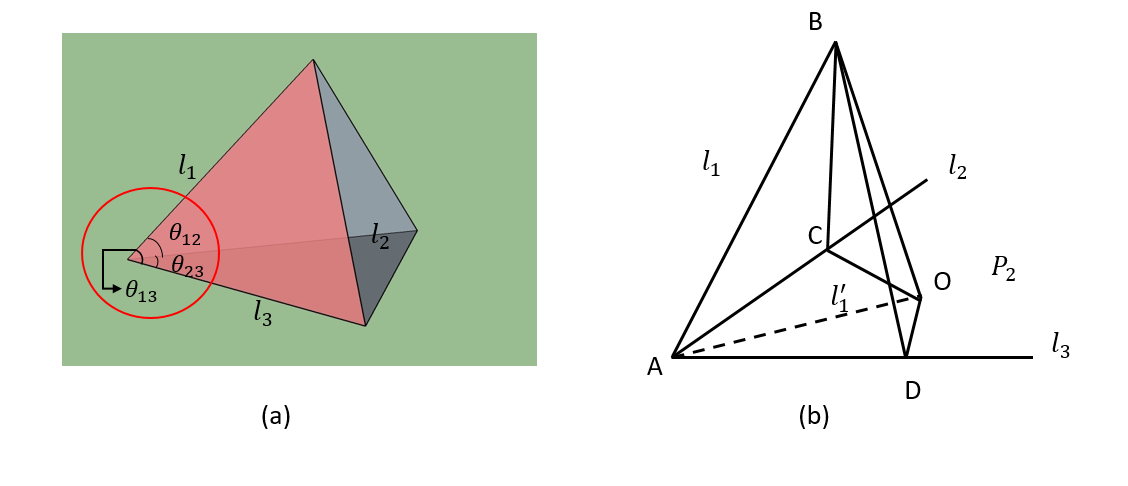
\includegraphics[width=3.0in]{images/peak.png}
%	\caption{Three rigid planes $P_1$, $P_2$, $P_3$ form a peak of a tetrahedron with their back face inside which is circled red in Figure \ref{fig:peak}(a), and we can proof its stability by constructing Figure \ref{fig:peak}(b)}
%	\label{fig:peak}
%\end{figure}


%\section{Algorithm}
%\subsection{Initiation??}
%
%\begin{description}
%	\item[Line Equality] if lines have equal length, they can probably be merged.
%	\item[Plane Parallelism] If there are only two planes which have equal area, this two are probably parallel to each other.
%\end{description}

%\section{Formulation}
%Simply put, our main problem is how to fold a planar layout $\mathcal{L} = \{l_i\}$ into its three-dimentional realization where $l_i$ represents $i$th line segment in the layout.Each line has a label that shows the line segment is solid or dashed which is used to cut or fold.
%
%Furthermore, we assume that every plane is rigid which means the interior angle in each plane stays the same, but planes can be bent during folding. Also, planes are connected by fold lines at the boundry of the patches, and we assume that the planar layout has its front and back.
%
%In order to slove this problem, we turn the box fold problem into triangular mesh deformation. One reason is that mesh can approximately represents both design layouts and 3D box models, thus we can turn this problem into functional mapping . Besides, the triangular mesh is widely studied and used, so we can use the Graph Laplacian as our methods, which will be mentioned in ****.
%
%\begin{figure}[ht]
%	\centering
%	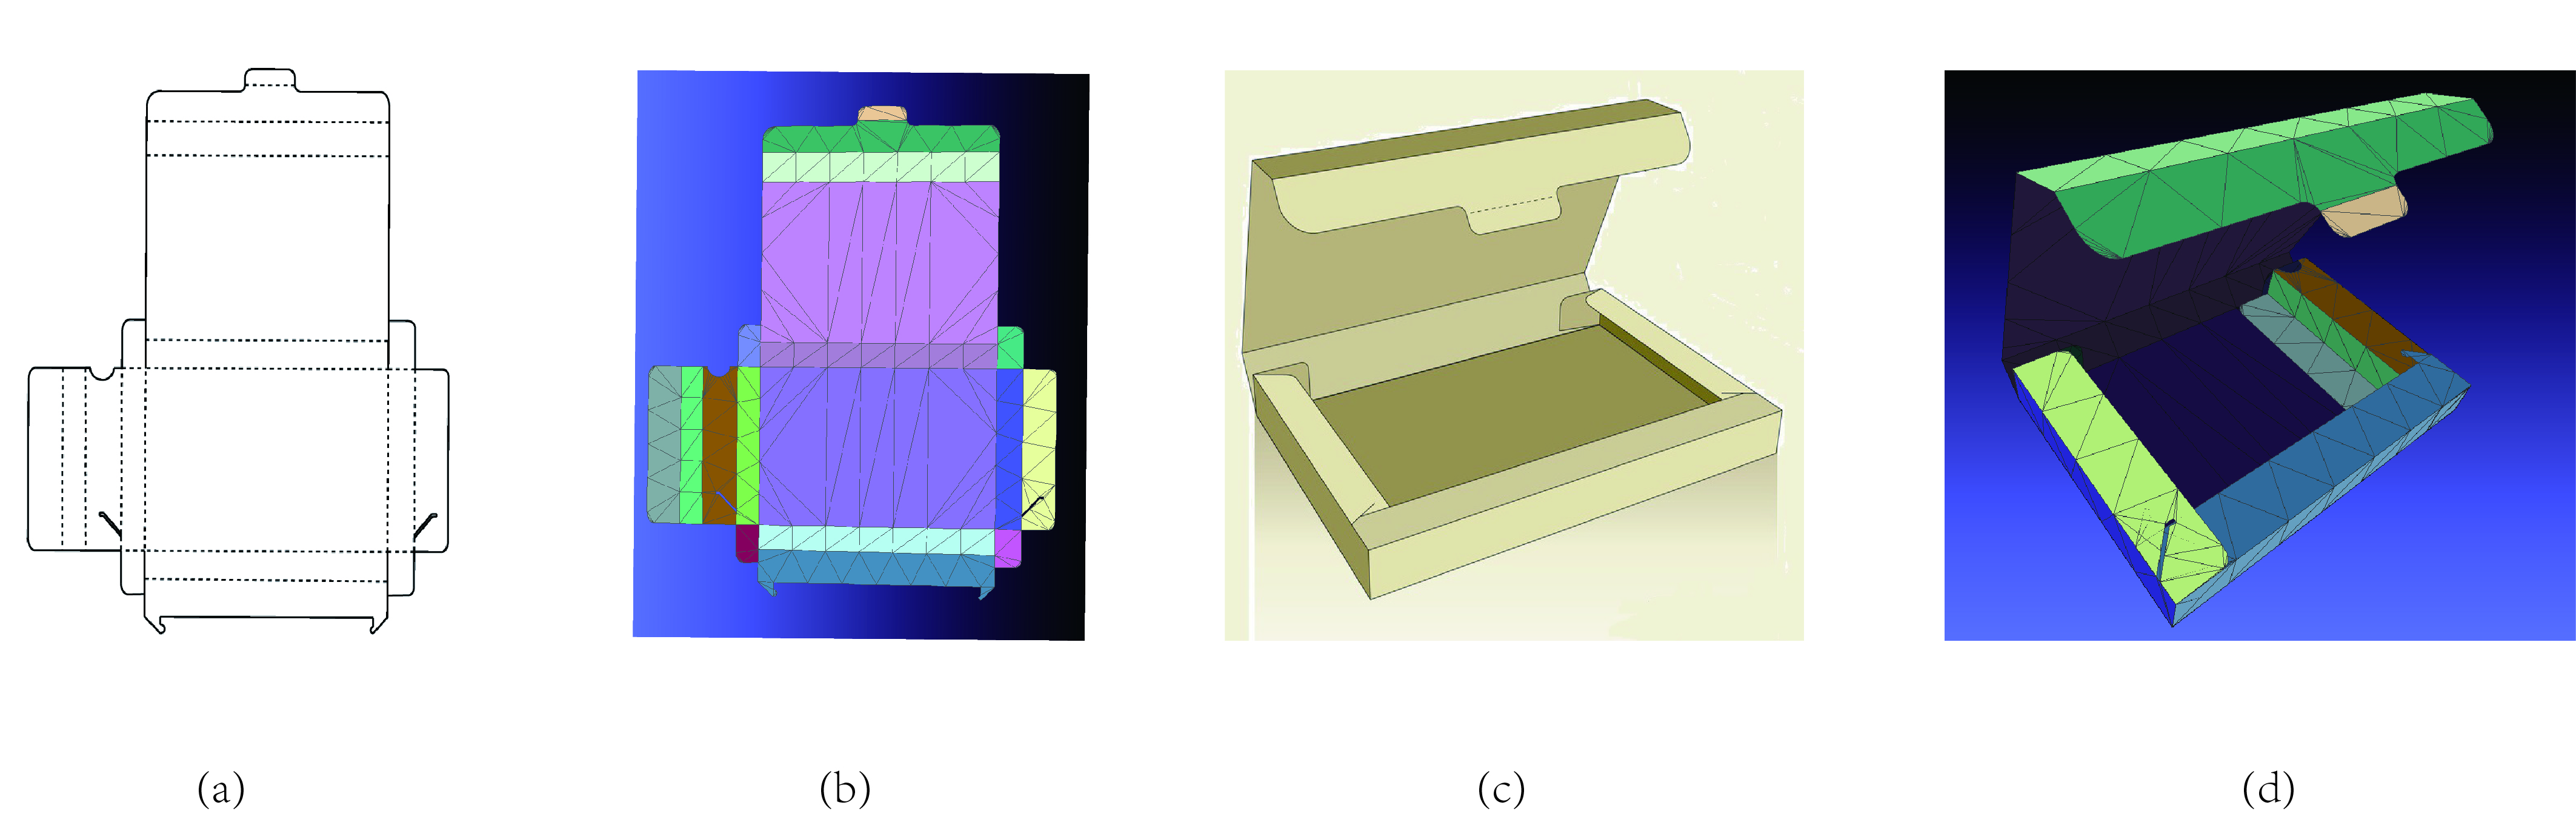
\includegraphics[width=3.0in]{images/approximation.jpg}
%	\caption{Given a design layout (a) and its 3D realization (c), we can approximately represent them by triangular mesh as (b) and (d).}
%	\label{fig:approximation}
%\end{figure}
%
%\subsection{New}
%If we assign the positive direction of normal is ***, and we know the final state of each angle, we can have the only one state of 3D realization. 
%
%\begin{equation}
%\theta: \{\mathbf{e_i}\}-> \{{\alpha_i}\} 
%\end{equation}
%
%\begin{equation}
%X_j: \{\mathbf{e_i}\}-> \mathbf{R}\\
%\end{equation}
%
%\begin{equation}
%F: \{X_1,X_2, \dots\}->\theta\\
%\end{equation}
%
%constrain:
%\begin{itemize}
%	\item $\alpha_i = \alpha_j$ if $\mathbf{e_i}$  and $\mathbf{e_j}$ are adjacent and paralleled, also they are in the same plane.??????(how to define)
%	\item $\alpha_i = \pi$ if $\mathbf{e_i}$ is inside the plane.??????(how to define)(does it appear?)
%\end{itemize}
%
%\subsubsection{Need to explain}
%\begin{itemize}
%	\item why a initial line sample to many short edges to learn more angles
%	\item bezier sample interval 
%\end{itemize}
%
%\subsubsection{Why laplacian can apply to our problem}
%Given a 2D flat mesh, we take each edge $\mathbf{e_i}$ as a graph node, and the distance function between two adjacent edges as its weight to construct a laplacian matrix $L = \{a_{i,j}\}$.
%\begin{equation}
%\left\{
%\begin{gathered}
%a_{i,j} = w_{i,j} = \exp^(-\frac{|dis|}{average dis}) \quad \hfill if (i,j) is adjacent. \\
%a_{i,i} = -\sum w_{i,j} \quad \hfill \\
%a_{i,j} = 0 \quad \hfill otherwise \\
%\end{gathered}
%\right.
%\end{equation}
%
%To some degree, the laplacian matrix can represent the layout structure, the eigenvectors and eigenvalues of the graph Laplacian contain both geometric and topological information, meanwhile the angles $\{\alpha_i\}$ we need to solve can been seen as a function $\theta$ defined in the layout $\mathcal{L}$.
%
%\begin{equation}
%\theta: \{\mathbf{e_i}\}-> \{{\alpha_i}\} 
%\end{equation}
%
%As a result, we can use the eigenvectors as basic functions to approximate the angle function $\theta$.
\section{Problem Formulation}
In this section we present the general concept of our learning approach. The basic idea is to interpret the folded state of a box as a series of rotation angles along each edge, where the problem of predicting folded state is turned into a problem of predicting these angles. 
\subsection{Definitions and Notations}
As an input to our method, we expect a 2D designed layout of a box represented as a flat triangular mesh $L$. As output of our method, we deform the input triangular mesh into its 3D realization $R$, according to predicted angles along each of its edges.(An example is shown in Figure~\ref{fig:approximation})\\
\begin{figure}
	\centering
	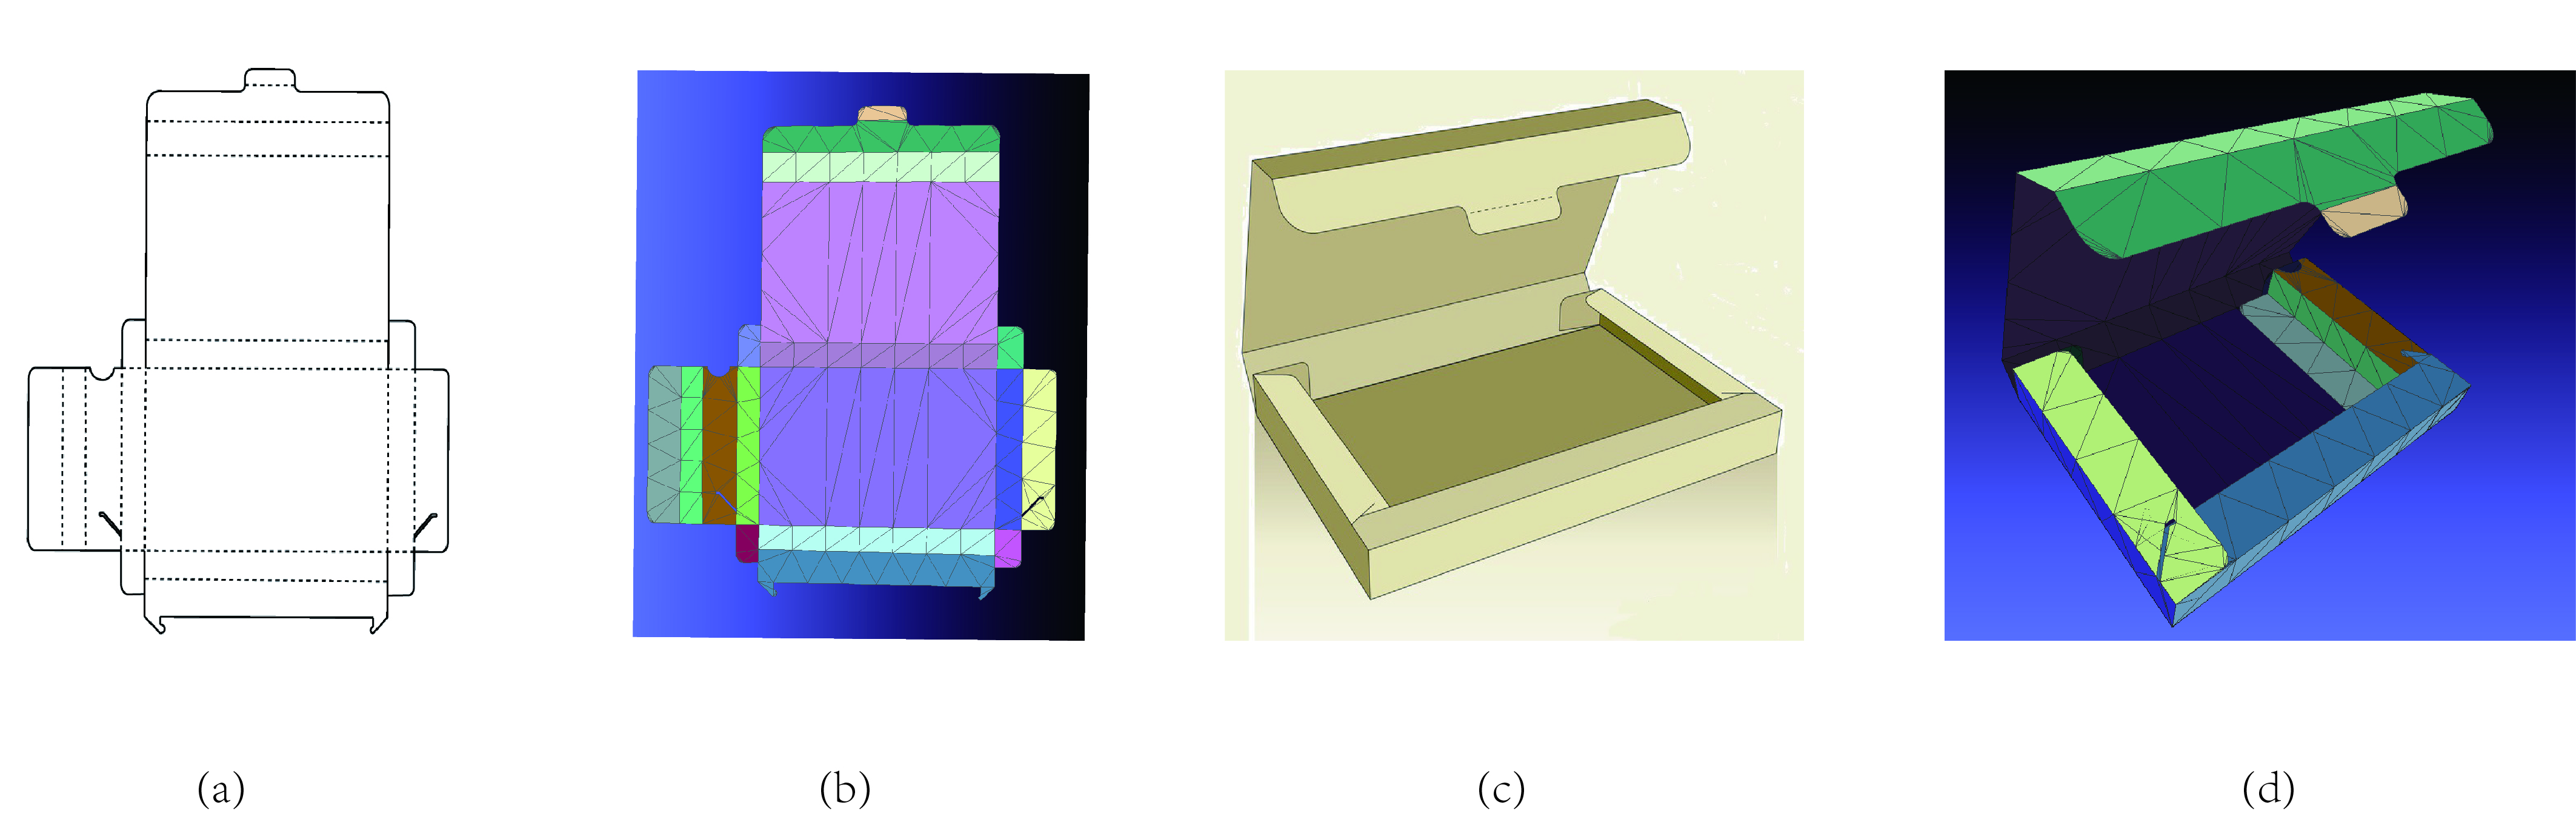
\includegraphics[width=3.0in]{images/approximation.jpg}
	\caption{Given a design layout (a) and its 3D realization (c), we can approximately represent them by triangular mesh as (b) and (d).}
	\label{fig:approximation}
\end{figure}
Without loss of generality, a learning approach should be able to learn an operator $F$ that maps every 2D layout to its 3D realization:
\begin{equation}
F:\{L\}\rightarrow\{R\}
\label{equ:F_0}
\end{equation}
in which $\{L\}$ is the set of all designed layout of boxes represented by 2D triangular meshes and $\{R\}$ is the set of 3D realization of the same boxes represented by deformed triangular meshes. For each triangular mesh 
\subsection{From Shape Mapping to Functional Mapping}
It is difficult to design a model and a learning scheme to learn the operator in (\ref{equ:F_0}).As we stressed before, the folded state of a box can be represented by a series of rotation angles along each edge.
\subsection{Choice of Features}
\subsection{Choice of Basis Functionals}


\section{Methods}

\input{experiment}

\section{User Study}

\section{Conclusion}

\section*{Acknowledgements}

To all.

\bibliographystyle{acmsiggraph}
\nocite{*}
\bibliography{ref}
\end{document}
